% Klassifiziert den Dokumenten-Typ
% Doku: http://exp1.fkp.physik.tu-darmstadt.de/tuddesign/
% Farben: http://www.tu-darmstadt.de/media/medien_stabsstelle_km/services/medien_cd/das_bild_der_tu_darmstadt.pdf
%  bigchapter: Chapter haben doppelte Schriftgröße
%  linedtoc: Linien im Inhaltsverzeichnis wie bei Überschriften
%  colorbacktitle: Der Dokumenten-Titel wird mir der Accentfarbe hinterlegt
\documentclass[bigchapter,colorback,accentcolor=tud4b,linedtoc,11pt]{tudreport}

% Input Dokument hat das Encoding UTF-8
\usepackage[utf8]{inputenc}
% Wichtiges Paket für Links und verlinktes Inhaltsverzeichnis
\usepackage[ngerman]{hyperref}
% Paket für Fußnoten
\usepackage[stable]{footmisc}
% Paket für amsmath (aligned mathe formeln)
\usepackage{amsmath}
% Paket für Bibliotheks-Verzeichnis, square: Verwende eckige statt runde klammern
% \usepackage[square]{natbib}
% Paket zum Plotten von Datensätzen
\usepackage{pgfplots}
\pgfkeys{
  /pgfplots/PolarStyle/.style={
    ylabel=Leistung in W,
    width=0.33\linewidth,
    height=0.33\linewidth,
    scale only axis,
    grid=both,
    tick align=outside,
    tickpos=left,
    minor x tick num=2,
    minor y tick num=1
  }
}

% Anhänge für Original-Messdaten
\usepackage{fancyvrb}

% redefine \VerbatimInput
\RecustomVerbatimCommand{\VerbatimInput}{VerbatimInput}%
{fontsize=\footnotesize,
 %
 frame=lines,  % top and bottom rule only
 framesep=2em, % separation between frame and text
 fontsize=\scriptsize,
 %
 labelposition=topline,
 %
 commandchars=\|\(\), % escape character and argument delimiters for
                      % commands within the verbatim
 commentchar=*        % comment character
}

% Polar Plots
\usetikzlibrary{pgfplots.polar}
% Verwende deutsche Bezeichner für Inhaltsverzeichnis, ... (ngerman = New German: neue Rechtschreibung)
\usepackage{ngerman}
% Deutsche Zahlen (entfernt z.B. das Leerzeichen nach einem Dezimal-Komma)
\usepackage{ziffer} 

\usepackage[verbose]{placeins}

%wegen Grafikverschiebung hinzugefügt
\usepackage{float}

%\usepackage{graphicx}
%\usepackage{caption}
\usepackage{subcaption} %Für subfigures

% PDF-Optionen
\hypersetup{
  pdftitle={TU Darmstadt \- Physikalisches Praktikum für Fortgeschrittene},
  pdfauthor={Esra Bauer und Sören Link},
  pdfsubject={Versuch 3.21},
  pdfview=FitH,
}
% Nummeriere formeln in Subsections einzeln
% Kleines makro zur assymetrischen Fehlerangabe

% Entspricht-Zeichen
\usepackage{scalerel}

\newcommand\equalhat{%
\let\savearraystretch\arraystretch
\renewcommand\arraystretch{0.3}
\begin{array}{c}
\stretchto{
    \scalerel*[\widthof{=}]{\wedge}
    {\rule{1ex}{3ex}}%
}{0.5ex}\\ 
=%
\end{array}
\let\arraystretch\savearraystretch
}
%BEGINN TITELSEITE

\title{Röntgenkleinwinkelstreuung an teilkristallinen Polymeren}

\subtitle{Esra Bauer  \\Sören Link}

\subsubtitle{Betreuer: Jan Gabriel \hfill Versuchsdatum: 24. November 2014}

\author{Esra Bauer, Sören Link}

%\settitlepicture{img/title.jpg}

\institution{Physikalisches Praktikum \\für Fortgeschrittene \\ Versuch 3.21}

\date{\today}


%ENDE TITELSEITE

\begin{document}
%ANFANG DOKUMENT

%Titelseite einfügen
\maketitle

%Inhaltsverzeichnis einfügen
\tableofcontents

%ANFANG INHALT

\chapter{Einleitung}

In diesem Versuch wird die Struktur von PET, einem Polymer, welches uns in Form von Getränkeflaschen bekannt ist, näher untersucht. Das Interessante dabei ist, dass es sich weder um einen rein amorhpen Stoff, wie z.B. Fensterglas oder auch andere Kunststoffe wie  Polystyrol (PS), Polyvinylchlorid (PVC) oder Polycarbonat (PC), noch um einen klassischen kristallinen Stoff handelt. Er besitzt vielmehr die Fähigkeit, sich teilweise kristallin zu ordnen, wobei dies stark von der Historie des Temperaturverlaufs abhängt. Daher werden im Versuch Proben des Materials untersucht, die unterschiedlich getempert wurden. Mithilfe der Röntgenkleinwinkelstreuung sollen Rückschlüsse auf die Struktur der Proben ermöglicht werden.

\chapter{Grundlagen}
\section{Polymere}

Allgemein handelt es sich bei Polymeren um Makromoleküle, die aus Kettenmolekülen oder verzweigten Molekülen aufgebaut sind. Diese Makromoleküle können aus bis zu mehreren hunderttausend Bausteinen bestehen, die man Monomere nennt. Die Länge der Polymere bestimmt dabei den Polymerisationsgrad und man unterscheidet Thermoplasten, Duroplasten und Elastomere, wobei bei ersteren die Makromoleküle kettenförmig sind, bei den Duroplasten stärker und bei Elastomeren schwächer vernetzt. Die physikalischen Eigenschaften sind dementsprechend unterschiedlich: Elastomere sind elastisch dehnbar und Duroplasten auch bei höheren Temperaturen starr bzw. im Vergleich eher spröde. 

Interessant sind für diesen Vesuch vor allem die Gruppe der Thermoplasten, zu denen auch das zu untersuchende PET gehört. Sie lassen sich, wie der Name sagt, einschmelzen und umformen. In der Schmelze liegen die Kettenmoleküle ungeordnet vor. Man spricht von einem Gaußschen Knäuel, da die Anordnung der Moleküle zufällig ist und in der Verteilung einer Gaußfunktion entspricht. Abhängig von der Abkühlgeschwindigkeit und -temperatur treten dann zwei wesentliche Übergänge auf: Der Glasübergang und (teilweise) Kristallisation.

\section{Glasübergang}

Kühlt man geschmolzene Thermoplasten schnell wieder ab, reicht die Zeit für die Kettenmoleküle, aus denen sie aufgebaut sind, nicht aus um sich regelmäßig anzuordnen, d.h. die Knäuelstruktur erstarrt und bleibt unregelmäßig. Es entsteht ein amorpher Festkörper, wie z.B. Fensterglas. Physikalisch handelt es sich dabei nicht um einen Phasenübergang, da keine fest definierte Temperatur für den Glasübergang existiert, sondern in der Realität ein allmählicher Übergang stattfindet, der zudem von der Abkühlgeschwindigkeit abhängt. Trägt man die zugeführte Wärme $Q_{zu}$ über der Temperatur T des Festkörpers auf, wird dies als Aufweichung sichtbar:


\begin{figure}[h] 
  \centering
     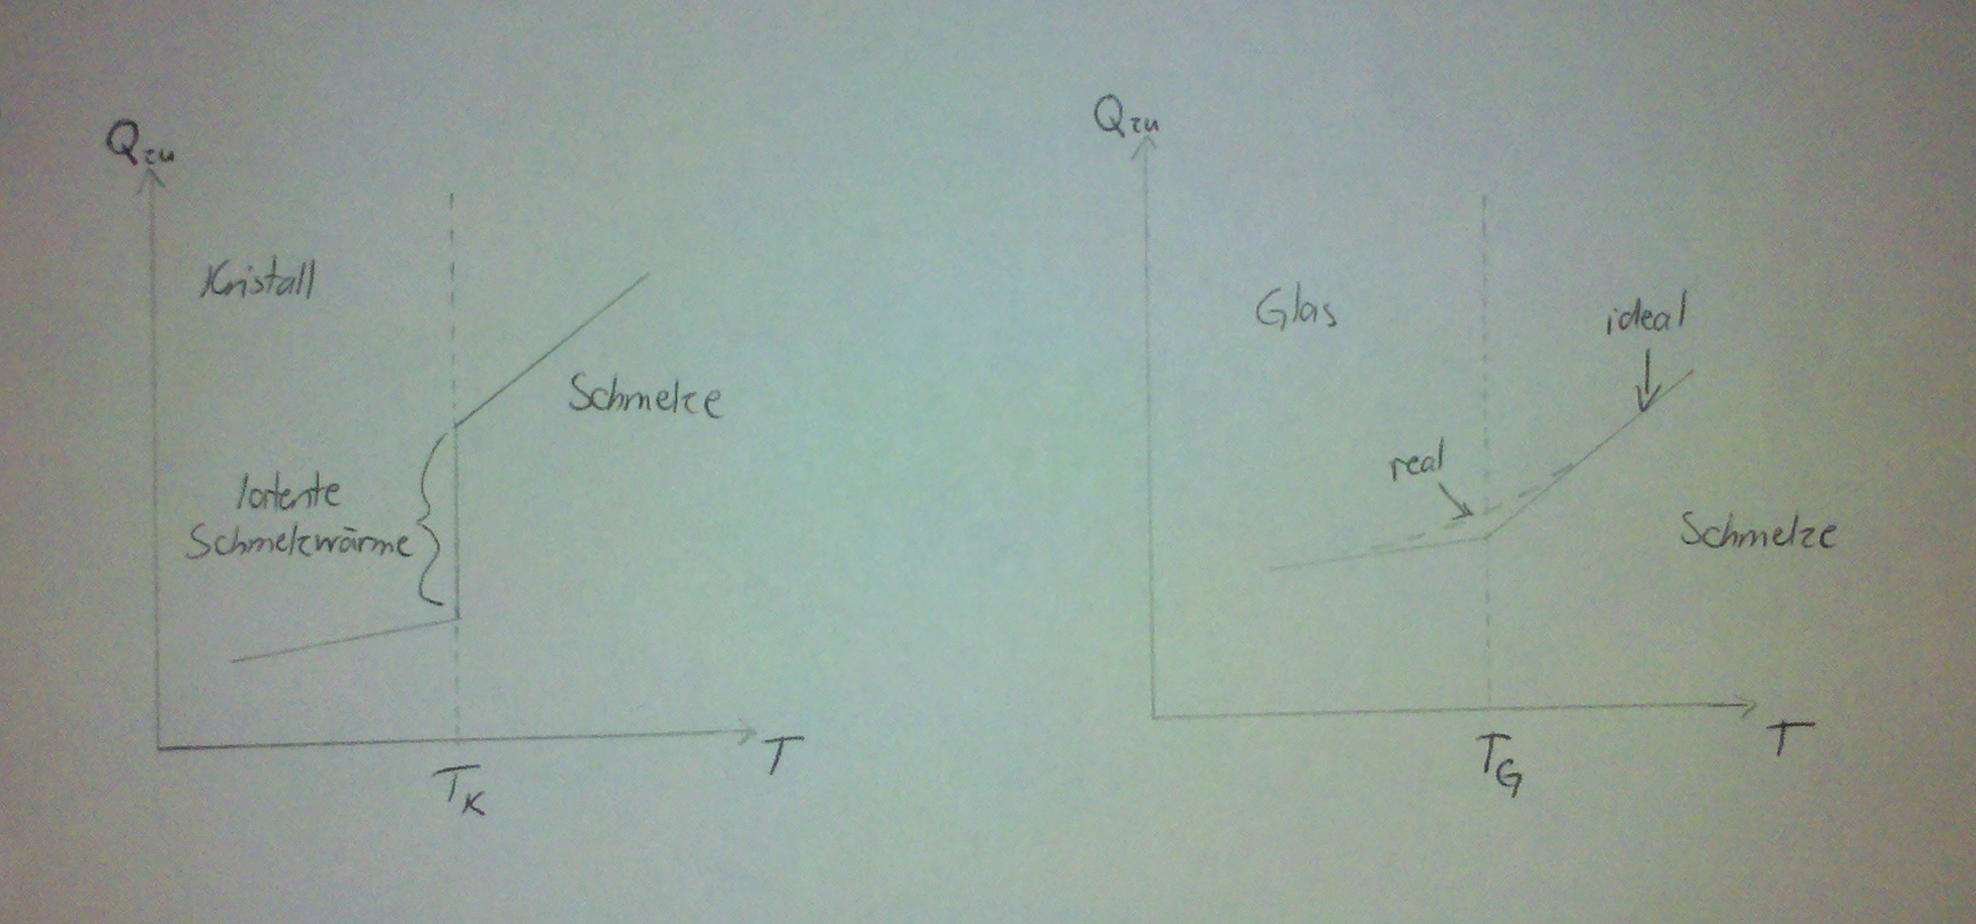
\includegraphics[width=0.7\textwidth]{data/glastemperatur.jpg}
  \caption{Zugeführte Wärme $Q_{zu}$ über der Temperatur des Festkörpers}
  \label{fig:Bild1}
\end{figure}

Im $Q_{zu}$-T-Diagramm kann der Glasübergang für eine ideale geringe Aufweichung der Glasübergangstemperatur allerdings wie ein Phasenübergang zweiter Ordnung erscheinen. Dennoch ist hier deutlich der Unterschied zum Kristallübergang, der ein Phasenübergang erster Ordnung ist, zu sehen. Charakteristisch für den Kristallübergang ist die latente Schmelzwärme, die sich nicht in einer Temperaturerhöhung zeigt, sondern für die Auflösung der kristallinen Strukturen benötigt wird. Am Diagramm für den Glasübergang wird auch deutlich, dass sich hieraus die Glasübergangstemperatur nur schwer bestimmen lässt. Eine alternative Methode hierfür ist deswegen die Zuordnung einer bestimmten Viskosität zur Glasübergangstemperatur.

\section{Kristallinität in Polymeren}

Wenn man die Abkühlgeschwindigkeit senkt bzw. den geschmolzenen Thermoplasten einige Zeit bei konstanter Temperatur hält und die Voraussetzung gegeben ist, dass die Kristallisationstemperatur höher als die Glasübergangstemperatur liegt, können die Kettenmoleküle sich gebietsweise regelmäßig strukturieren. Man spricht dann von Kristallisation. Energetisch am günstigen wäre ein Zustand, in dem sämtliche Ketten vollständig entfaltet parallel aneinanderliegen würden. Dies lässt sich dadurch erklären, dass zwischen den Ketten Van-der-Waals-Kräfte wirken, die vor allem bei kleinem Teilchenabstand zum Tragen kommen und bei größerem Abstand vernachlässigbar schwach werden. Folglich erfährt eine Kette, die nicht parallel zur nächsten liegt, in der Regel Kräfte verschiedener anderer Ketten in verschiedene Richtungen, d.h. der Zustand ist nicht stabil. Liegen die Ketten allerdings parallel, wird die Van-der-Waals-Kraft pro Kette auf ihren Nachbarn maximal, da jedes Teilchen den kleinstmöglichen Abstand zum entsprechenden Teilchen der Nachbarkette hat.

Zunächst erfolgt eine Keimbildung, d.h. es bilden sich sog. Kristallite (lokale Ordnungszustände mit einer typischen Größe von 15-100 nm), in denen die Molekülketten großteils parallel liegen. Großteils deshalb, weil sich die langen Molekülketten, obwohl dies energetisch am günstigsten wäre, nicht vollständig entfalten können. In der Realität falten sich die Ketten und liegen an den Enden und Schlaufen oft ungeordnet vor. Diese Kristallite können nun weiter wachsen, wobei zu beachten ist, dass sie dies bevorzugt in eine ausgezeichnete Richtung tun, da zum einen an den Seiten, an denen die Schlaufen liegen, kein Wachstum stattfinden kann, da hier amporhe Bereiche außenliegend sind, und zum andern die Richtung des größten Temperaturgradienten bevorzugt wird. Somit wächst der Kristallit in die Länge, es entstehen sog. Lamellen, also längliche Kristallstrukturen, in denen die Molekülketten quer zur Längsachse der Lamellen angeordnet sind.

Beim weiteren Wachstum muss unterschieden werden, unter welchem Temperaturbedingungen die Kristallisation erfolgt. Besteht ein starkes Temperaturgefälle, ordnen sich die Lamellen parallel an. Dies ist aber im Rahmen des Versuchs nicht weiter von Belang, da die Proben unter weitgehend isotropen Temperaturbedingen kristallisiert wurden, wobei sich die Lamellen radialsymmetrisch anordnen. Man spricht bei diesen radialsymmetrischen Strukturen von Sphärolithen. Eine vollständige Kristallisation ist in Polymeren nicht möglich, da bereits die Grundbausteine, die Kristallite, amorphe Randbereiche besitzen, an denen sich keine geordnete Struktur anlagern kann. Die Kristallisation lässt sich aber durch Additive signifikant steigern, auch Verunreinigungen und nicht ganz aufgeschmolzene kristalline Bestandteile können die Kristallisation verbessern.

\section{Röntgenstreuung}
TODO: Funktionsweie Röntgenröhren, Peaks, Streuung (Amplitude, Intensität, Furier, Autokorrelationsunfktion, Elektronendichte)

Unter Röntgenstrahlung versteht man elektromagnetische Strahlung hoher Energie (zwischen 100 eV und einigen MeV), deren Wellenlängen entsprechend zwischen 10$^{-12}$ und 10$^{-8}$ liegen. Sie lässt sich beispielsweise mit einem Synchrotron oder einer Röntgenröhre erzeugen, wobei im Folgenden letztere verwendet wird und daher hier kurz auf die Funktionsweise eingegangen werden soll. Im Wesentlichen besteht die Röntgenröhre aus einer beheizten Kathode, die freie Elektronen erzeugt, sowie aus einer Anode, die gegenüber der Kathode eine Hochspannung von 40kV besitzt. Die Elektronen werden also zur Anode beschleunigt, was in zwei Arten von Strahlung resultiert, da zum einen Wechselwirkung der Elektronen mit dem elektromagnetischen Feld der Anode stattfindet, wobei die Elektronen abgelenkt bzw. gebremst werden (dies verursacht ein kontinuierliches Spektrum der sog. Bremsstrahlung), und zum andern die energiereicheren Elektronen Hüllenelektronen aus dem Anodematerial herausschlagen können. Der Effekt ist, dass ein Hüllenelektron der nächsten Schale nachrückt und genau die Energiedifferenz der beiden Schalen in Form von elektromagnetischer Strahlung frei wird. Es entsteht zusätzlich ein diskretes Spektrum der charakteristischen Röntgenstrahlung. Ein Übergang der L-Schale zur K-Schale wird dabei als $K_{\alpha}$-Linie bezeichnet, ein Übergang der M-Schale zur K-Schale als $K_{\beta}$-Linie usw. Die Lage der Linien sind dabei vom Anodenmaterial abhängig, welches in diesem Fall Kupfer ist. 

Alle Messungen werden mit einer sog. Kratky-Kompakt-Kamera durchgeführt. Sie besteht aus einem evakuierbaren Gehäuse (Betriebsdruck ca. 38 mbar), welches einseitig auf der Röntgenröhre aufliegt und an der anderen Seite einen per Schrittmotor fein verschiebbaren Szintillationsdetektor vorgeschaltet hat. An beiden Enden ist das Gehäuse mit 0,25 mm dicken Berylliumfenstern verschlossen, die der Röntgenstrahl durchdringt. Vor der Strahlungsquelle befindet sich zunächst das Kollimationssystem, ein sog. Blockkollimationssystem, welches aus drei rechteckigen, genau geschliffenen Blöcken besteht, wobei zwei Blöcke den Strahl nach oben begrenzen und einer nach unten. Der Strahl passiert zuerst den Eingangspalt (dies ist der vertikale Abstand der in Strahlrichtung ersten beiden Blöcke, welcher auf etwa 80 µm eingestellt wird) und danach den letzten oberen Block, welcher gemeinsam mit dem mittleren Block die Strahlebenen bestimmt und Streustrahlung unterdrückt. So kollimiert, trifft der Strahl auf die Probe (bzw. passiert bei der ersten Messung den leeren Probenhalter) und wird dann auf das Austrittsfenster gestreut. Bei den Messungen mit Probe wird der Primärstrahl, d.h. der nicht gestreute Strahl, durch einen metallenen Beamstop blockiert, um ein direktes Auftreffen auf den Detektor zu verhindern, da dieser dadurch zerstört werden würde. Der Abstand der Probe zum Detektor beträgt 20 cm.

\section{Streuung an zweiphasigen Schichtsystemen}
TODO: Autokorrelationsfunktion, Invariante Q, Herleitung (wie in vorbesprechung), Abweichung Tatsächliche Korrelationsfunktion von einer für ein idealisiertes System


\chapter{Durchführung}
\section{Präparation der PET-Probe}

Bei dem Material, welches in diesem Versuch untersucht wird, handelt es sich um Polyethylenterephtalat (PET), welches man in Form von Getränkeflaschen kennt und auch für die Herstellung von Folien und Fasern verwendet wird. Wir bedienen uns einer handelsüblichen PET-Flasche und schneiden kleine Stücke passend für den Probenhalter aus. Der Probenhalter ist ein längs geteiler Messingzylinder, in dessen Mitte ein längliches Messingplättchen einer Stärke von 1 mm mit rechteckiger Aussparung verschraubt wird. In dieser Aussparung fixieren und schmelzen/kristallisieren wir unsere Probe. Zur Fixierung dient Aluminiumfolie, die einmal um das Plättchen herumgelegt wird, nachdem das PET-Rohmaterial eingelegt worden ist. Nun legen wir das Plättchen auf eine Kochplatte und lassen es einige Zeit bei knapp unter 300 $^{\circ}$C schmelzen. Anschließend kommt die Probe für 10 Minuten (per Stoppuhr genau überprüft) bei 170 $^{\circ}$C in einen Ofen, um sie kristallisieren zu lassen. Nach Ablauf der 10 Minuten wird sie in kaltem Wasser abgeschreckt und ist nun nach Abtrocknung zur Messung bereit. 

Bei der Schmelze ist zu beachten, dass das PET verläuft und man deswegen die Menge nicht zu reichlich bemessen sollte, da es sonst aus der Aussparung überläuft, was in der Tat auch beinahe geschehen ist. Zudem hat sich gegen Ende der Schmelze eine bräunliche Verfärbung eingestellt, was zwei Gründe haben kann; zum einen hat der Schmelzvorgang deutlich länger angedauert als im Anleitungsblatt empfohlen, zum andern ist die Temperatur teilweise knapp über 300 $^{\circ}$C angestiegen. Zur Schmelzdauer ist zu sagen, dass die im Anleitungsblatt empfohlenen 5 Minuten etwas knapp bemessen sind, da die Wärmeleitung zwischen der Heizplatte und dem Probenhalter dazu nicht ausreicht, allerdings hat die tatsächliche Schmelze etwa 45 Minuten angedauert, was vermutlich wiederum zu lang ist (ideal sollten ca. 15-20 Minuten sein). Um die Temperatur konstant zu halten, ist es außerdem erforderlich, die Heizleistung der Platte nachzuregeln, u.a. wohl deswegen, weil zur Fixierung des Temperatursensors ein Ziegelstein auf der Platte liegt, der sich erst nach und nach aufheizt und zu Anfang deshalb mehr Heizleistung aufnimmt. Selbiges gilt auch für die übrigen Materialien, die mit aufgeheizt werden (metallene Heizplatte, Probenhalter usw.).

\section{Bestimmung des Primärstrahlprofils}

Vor Beginn der eigentlichem Messung ist es notwendig, die Intensitätsverteilung des Primärstrahls zu bestimmen, da die Strichkollimation zwar gegenüber der Punktkollimation den Vorteil der generell höheren Intensität besitzt, jedoch das Strahlprofil nicht genau rechteckig ist, sondern abgerundet und zu den Rändern allmählich ausläuft. Aus diesem Grund müssen wir also zuerst eine Messung ohne Probe und ohne Primärstrahlfänger durchführen. Da ohne weitere Maßnahmen damit der empfindliche Szintillitationsdetektor zerstört werden würde, schalten wir den Messingabsorber vor die Strahlungsquelle dazu, der Strahl wird insgesamt also stark abgeschwächt. Zusätzlich montieren wir einen horizontalen Spalt mit einer Breite von 200 µm vor den Detektor. Das Innere der Kratky-Kamera wird anschließend evakuiert und eine winkelabhängige Messung der Intensität gestartet. 

Zuletzt setzen wir den Nullpunkt des Detektors auf das eben bestimmte Maximum des Primärstrahls, um die folgenden Messungen relativ dazu betrachten zu können.

\section{Hintergrundmessung mit leerem Probenhalter und Aluminiumfolie}

Um aus späteren Messungen die vom Probenbehlter und der Aluminiumfolie verursachte Hintergrundstrahlung herausrechnen zu können, war es notwendig, eine Messreihe mit einem leeren Probenbehälter durchzuführen. Dazu wurde der leere, mit Aluminiumfolie umwickelter, Probenbehälter in der Apparatur installiert, die Kratky-Kamera evakuiert und erneut eine winkelabhängige Messung der Intensität gestartet. Im Gegensatz zur Bestimmung des Primärstrahlprofils messen wir hier allerdings nur die gestreute Röntgenstrahlung, es wird also kein Absorber zur Abschwächung des Primärstrahls verwendet. Um dabei das Szintillatormessgerät nicht zu beschädigen, wird ein Primärstrahlfänger angebracht. Dieser ist so angebracht, dass der nicht abgelenkte Primärstrahl vollständig geblockt wird, die gestreute Strahlung allerdings ungehindert in den Szintillator eindringen kann.

Die Original-Messdaten für diese Messung sind als "`Untergrund.0.txt"' angehängt.

\subsection{Wanderspaltmessung}
Zur Entschmierung der einzelnen Streudatenmessungen ist es notwendig, noch eine sogenannte Wanderspaltmessung durchzuführen. Dabei wird der zuvor angebrachte Horizontaler $200\mu m$ Spalt durch einen ebenfalls unbeweglichen $32 \mu m$ breiten vertikalen Spalt ausgetauscht. Zusätzlich wird vor der Probe ein beweglicher Spalt eingebracht. Dieser fährt in einem Zeitraum von 10 Sekunden von einer Seite des Primärstrahls zur anderen und anschließend mit gleicher Geschwindigkeit wieder zurück. Da bei dieser Messmethode nur ein sehr kleiner Teil der Strahlung beide Spalte passieren kann und statt der gestreuten Strahlung die Intensität des Primärstrahls gemessen wird, muss für die Wanderspaltmessung der Primärstrahlfänger entfernt werden.

Die Messung der Intensität erfolgt hierbei nicht winkelabhängig, statdessen wird pro Messung die Intensität des Primärstrahls über die gesamten 20 Sekunden aufgenommen den der bewegliche Spalt braucht, um wieder in die Startposition zurückzukehren.

Um den Fehler der Messung (Verursacht durch die statistische Natur der emittierten Röntgenstrahlung oder nicht gleichzeitigen Startens der Messung und des Spaltmotors) zu reduzieren, wird für jede Probe die Wanderspaltmessung 5 mal durchgeführt.

Die Original-Messdaten für diese Messung sind als "`Alu.ms"' angehängt.

\section{Messungen mit Probe}
Analog zur winkelabhängigen- und Wanderspaltmessung mit der leeren Probe haben wir die Intensität des Primärstrahls mit der Wanderspalt-Messmethode sowie die winkelabhängige Intensität der gestreuten Strahlung für jede der uns zur Verfügung stehendenden Proben gemessen. Dabei ist anzumerken, dass bei der Messung der ersten Probe die Röntgenröhre ausgeschaltet war. Die Ursache für die Abschaltung ist uns nicht genau bekannt, eventuell ist jemand trotz aller Vorsicht versehentlich gegen den gelben Strom-Schalter für die Röntgenröhre gekommen.

Weiterhin wurde bei der Wanderspaltmessung wiederholt die Verbindung zwischen Messgerät und dem zur Auswertung benutzten Computer getrennt. Dies wurde vermutlich durch eine kleine Spannungsspitze beim Ein- oder Ausschalten des Motors für den beweglichen Spalt verursacht.

Die einzelnen Messungen wurde von uns in folgender Reihenfolge durchgeführt:


\begin{center}
  \begin{tabular}{|p{2.2cm}|p{4.5cm}|p{3cm}|p{4cm}|}
    \hline
    Messungs-Nummer & Kristallisationstemperatur der Probe in °C & Messmethode    & Name der Messdaten-Datei \\ \hline
    1               & 140                                        & Winkelabhängig & PET-140.0.txt \\ \hline
    2               & 140                                        & Wanderspalt    & PET-140.ms \\ \hline
    3               & 170                                        & Wanderspalt    & PET-170.ms \\ \hline
    4               & 170                                        & Winkelabhängig & PET-170.0.txt \\ \hline
    5               & 170 (Selbst getempert)                     & Winkelabhängig & PET-170-eigen.0.txt \\ \hline
    6               & 170 (Selbst getempert)                     & Wanderspalt    & PET-170-eigen.ms \\ \hline
    7               & 200                                        & Wanderspalt    & PET-200.ms \\ \hline
    8               & 200                                        & Winkelabhängig & PET-200.0.txt \\ \hline
    9               & 215                                        & Winkelabhängig & PET-215.0.txt \\ \hline
    10              & 215                                        & Wanderspalt    & PET-215.ms \\ \hline
	\end{tabular}
\end{center}

\chapter{Auswertung}
\section{Strahlcharakterisierung}

Folgende Grafik zeigt die Verteilung der Messereignisse in Abhängigkeit der vertikalen Detektorposition. Durch den horizontalen Spalt von 200 µm vor dem Detektor kann die Verteilung sehr genau über der Position aufgelöst werden. Wie zu sehen ist, liegt das Maximum bei 2050 µm und die Abnahme der Intensität ist nicht genau symmetrisch.

\begin{center}
\begin{figure}[h]
\begin{tikzpicture}
\begin{axis}[
    legend pos=south west,
    title={Messereignisse in Abhängigkeit der Detektorposition},
    xlabel=Detektorposition in µm,
    x tick label style={/pgf/number format/1000 sep=},
    ylabel=Messereignisse,
    y tick label style={/pgf/number format/1000 sep=},
    width=0.9\textwidth,
    height= 9cm,
    xmin=1500,
    xmax=2500,
    grid=both,
    ymin=0,
    %ymax=0.0045,
    tick align=outside,
    tickpos=left,
    minor x tick num=3,
    minor y tick num=4,
    minor grid style={dotted,thin}
]
\addplot[red, only marks, mark=x, mark size=1pt, %error bars/.cd, y dir=both, y fixed relative=0.01, x dir=both, x fixed=0.05
]
table[x index={0},y index={1}] {data/beamprofile2.bp};
%\addlegendentry{Leistung der LED auf der Photoplatte}
\end{axis}
\end{tikzpicture}
\captionof{figure}{Zahl der Messereignisse über der Detektorpositon mit leeren Probenhalter, ohne beamstop und mit Messing-Strahlabsorber.}
\end{figure}
\end{center}

\section{PET-Streudaten}
TODO: Rohdaten, Entschmierung, Intensität vs. Streuvektor, Langperiode abschätzen

\section{Eindimensionale Korrelationsfunkton}
TODO: Berechnung/Darstellung von K(Z), Kristallinität, Langperiode, Kristallicke, Zusammenhang mit Temperatur, Vergleich mit Theorie

\chapter{Fazit}
TODO: Fazit, mögliche Verbesserungen (Herstellung der Probe?)

%ENDE INHALT
\cleardoublepage{}
% Eintrag fürs Inhaltsverzeichnis
\newpage
\begin{thebibliography}{100}
  \bibitem{GefahrenLaser} \url{http://de.wikipedia.org/w/index.php?title=Laser&oldid=128632514#Gefahren}
\end{thebibliography}

\chapter{Messdaten}
\VerbatimInput[label=\fbox{beamprofile.bp}]{data/beamprofile.bp}
\VerbatimInput[label=\fbox{untergrund.0.txt}]{data/untergrund.0.txt}
\VerbatimInput[label=\fbox{Alu.ms}]{data/Alu.ms}
\VerbatimInput[label=\fbox{PET-140.0.txt}]{data/PET-140.0.txt}
\VerbatimInput[label=\fbox{PET-140.ms}]{data/PET-140.ms}
\VerbatimInput[label=\fbox{PET-170.0.txt}]{data/PET-170.0.txt}
\VerbatimInput[label=\fbox{PET-170.ms}]{data/PET-170.ms}
\VerbatimInput[label=\fbox{PET-170-eigen.0.txt}]{data/PET-170-eigen.0.txt}
\VerbatimInput[label=\fbox{PET-170-eigen.ms}]{data/PET-170-eigen.ms}
\VerbatimInput[label=\fbox{PET-200.0.txt}]{data/PET-200.0.txt}
\VerbatimInput[label=\fbox{PET-200.ms}]{data/PET-200.ms}
\VerbatimInput[label=\fbox{PET-215.0.txt}]{data/PET-215.0.txt}
\VerbatimInput[label=\fbox{PET-215.ms}]{data/PET-215.ms}
\cleardoublepage{}
% Eintrag fürs Inhaltsverzeichnis
% Abbildungsverzeichnis einfügen
\end{document}
